%  LaTeX support: latex@mdpi.com
%  In case you need support, please attach all files that are necessary for compiling as well as the log file, and specify the details of your LaTeX setup (which operating system and LaTeX version / tools you are using).

%=================================================================
\documentclass[Agronomy,article,submit,moreauthors,pdftex]{mdpi}

% If you would like to post an early version of this manuscript as a preprint, you may use preprint as the journal and change 'submit' to 'accept'. The document class line would be, e.g., \documentclass[preprints,article,accept,moreauthors,pdftex]{mdpi}. This is especially recommended for submission to arXiv, where line numbers should be removed before posting. For preprints.org, the editorial staff will make this change immediately prior to posting.

%% Some pieces required from the pandoc template
\setlist[itemize]{leftmargin=*,labelsep=5.8mm}
\setlist[enumerate]{leftmargin=*,labelsep=4.9mm}


%--------------------
% Class Options:
%--------------------
%----------
% journal
%----------
% Choose between the following MDPI journals:
% acoustics, actuators, addictions, admsci, aerospace, agriculture, agriengineering, agronomy, algorithms, animals, antibiotics, antibodies, antioxidants, applsci, arts, asc, asi, atmosphere, atoms, axioms, batteries, bdcc, behavsci , beverages, bioengineering, biology, biomedicines, biomimetics, biomolecules, biosensors, brainsci , buildings, cancers, carbon , catalysts, cells, ceramics, challenges, chemengineering, chemistry, chemosensors, children, cleantechnol, climate, clockssleep, cmd, coatings, colloids, computation, computers, condensedmatter, cosmetics, cryptography, crystals, dairy, data, dentistry, designs , diagnostics, diseases, diversity, drones, econometrics, economies, education, electrochem, electronics, energies, entropy, environments, epigenomes, est, fermentation, fibers, fire, fishes, fluids, foods, forecasting, forests, fractalfract, futureinternet, futurephys, galaxies, games, gastrointestdisord, gels, genealogy, genes, geohazards, geosciences, geriatrics, hazardousmatters, healthcare, heritage, highthroughput, horticulturae, humanities, hydrology, ijerph, ijfs, ijgi, ijms, ijns, ijtpp, informatics, information, infrastructures, inorganics, insects, instruments, inventions, iot, j, jcdd, jcm, jcp, jcs, jdb, jfb, jfmk, jimaging, jintelligence, jlpea, jmmp, jmse, jnt, jof, joitmc, jpm, jrfm, jsan, land, languages, laws, life, literature, logistics, lubricants, machines, magnetochemistry, make, marinedrugs, materials, mathematics, mca, medicina, medicines, medsci, membranes, metabolites, metals, microarrays, micromachines, microorganisms, minerals, modelling, molbank, molecules, mps, mti, nanomaterials, ncrna, neuroglia, nitrogen, notspecified, nutrients, ohbm, particles, pathogens, pharmaceuticals, pharmaceutics, pharmacy, philosophies, photonics, physics, plants, plasma, polymers, polysaccharides, preprints , proceedings, processes, proteomes, psych, publications, quantumrep, quaternary, qubs, reactions, recycling, religions, remotesensing, reports, resources, risks, robotics, safety, sci, scipharm, sensors, separations, sexes, signals, sinusitis, smartcities, sna, societies, socsci, soilsystems, sports, standards, stats, surfaces, surgeries, sustainability, symmetry, systems, technologies, test, toxics, toxins, tropicalmed, universe, urbansci, vaccines, vehicles, vetsci, vibration, viruses, vision, water, wem, wevj

%---------
% article
%---------
% The default type of manuscript is "article", but can be replaced by:
% abstract, addendum, article, benchmark, book, bookreview, briefreport, casereport, changes, comment, commentary, communication, conceptpaper, conferenceproceedings, correction, conferencereport, expressionofconcern, extendedabstract, meetingreport, creative, datadescriptor, discussion, editorial, essay, erratum, hypothesis, interestingimages, letter, meetingreport, newbookreceived, obituary, opinion, projectreport, reply, retraction, review, perspective, protocol, shortnote, supfile, technicalnote, viewpoint
% supfile = supplementary materials

%----------
% submit
%----------
% The class option "submit" will be changed to "accept" by the Editorial Office when the paper is accepted. This will only make changes to the frontpage (e.g., the logo of the journal will get visible), the headings, and the copyright information. Also, line numbering will be removed. Journal info and pagination for accepted papers will also be assigned by the Editorial Office.

%------------------
% moreauthors
%------------------
% If there is only one author the class option oneauthor should be used. Otherwise use the class option moreauthors.

%---------
% pdftex
%---------
% The option pdftex is for use with pdfLaTeX. If eps figures are used, remove the option pdftex and use LaTeX and dvi2pdf.

%=================================================================
\firstpage{1}
\makeatletter
\setcounter{page}{\@firstpage}
\makeatother
\pubvolume{xx}
\issuenum{1}
\articlenumber{5}
\pubyear{2019}
\copyrightyear{2019}
%\externaleditor{Academic Editor: name}
\history{Received: date; Accepted: date; Published: date}
\updates{yes} % If there is an update available, un-comment this line

%% MDPI internal command: uncomment if new journal that already uses continuous page numbers
%\continuouspages{yes}

%------------------------------------------------------------------
% The following line should be uncommented if the LaTeX file is uploaded to arXiv.org
%\pdfoutput=1

%=================================================================
% Add packages and commands here. The following packages are loaded in our class file: fontenc, calc, indentfirst, fancyhdr, graphicx, lastpage, ifthen, lineno, float, amsmath, setspace, enumitem, mathpazo, booktabs, titlesec, etoolbox, amsthm, hyphenat, natbib, hyperref, footmisc, geometry, caption, url, mdframed, tabto, soul, multirow, microtype, tikz

%=================================================================
%% Please use the following mathematics environments: Theorem, Lemma, Corollary, Proposition, Characterization, Property, Problem, Example, ExamplesandDefinitions, Hypothesis, Remark, Definition
%% For proofs, please use the proof environment (the amsthm package is loaded by the MDPI class).

%=================================================================
% Full title of the paper (Capitalized)
\Title{Identification of high-yielding soybean lines with exceptional
seed composition qualities}

% Authors, for the paper (add full first names)
\Author{Jay
Gillenwater$^{1,\ddagger,*}$\href{https://orcid.org/0000-0002-3477-6291}{\orcidicon}}

% Authors, for metadata in PDF
\AuthorNames{Jay Gillenwater}

% Affiliations / Addresses (Add [1] after \address if there is only one affiliation.)
\address{%
$^{1}$ \quad Department of Crop and Soil Sciences, NCSU, Raleigh, NC,
USA; \href{mailto:jhgille2@ncsu.edu}{\nolinkurl{jhgille2@ncsu.edu}}\\
}
% Contact information of the corresponding author
\corres{Correspondence: \href{mailto:leutnant@fh-muenster.de}{\nolinkurl{leutnant@fh-muenster.de}};
Tel.: +XX-000-00-0000.}

% Current address and/or shared authorship
\firstnote{Current address: Updated affiliation}
\secondnote{These authors contributed equally to this work.}






% The commands \thirdnote{} till \eighthnote{} are available for further notes

% Simple summary
\simplesumm{A Simple summary goes here.}

% Abstract (Do not insert blank lines, i.e. \\)
\abstract{A single paragraph of about 200 words maximum. For research
articles, abstracts should give a pertinent overview of the work. We
strongly encourage authors to use the following style of structured
abstracts, but without headings: 1) Background: Place the question
addressed in a broad context and highlight the purpose of the study; 2)
Methods: Describe briefly the main methods or treatments applied; 3)
Results: Summarize the article's main findings; and 4) Conclusion:
Indicate the main conclusions or interpretations. The abstract should be
an objective representation of the article, it must not contain results
which are not presented and substantiated in the main text and should
not exaggerate the main conclusions.}

% Keywords
\keyword{yield; protein; oil;soybean; protein meal}

% The fields PACS, MSC, and JEL may be left empty or commented out if not applicable
%\PACS{J0101}
%\MSC{}
%\JEL{}

%%%%%%%%%%%%%%%%%%%%%%%%%%%%%%%%%%%%%%%%%%
% Only for the journal Diversity
%\LSID{\url{http://}}

%%%%%%%%%%%%%%%%%%%%%%%%%%%%%%%%%%%%%%%%%%
% Only for the journal Applied Sciences:
%\featuredapplication{Authors are encouraged to provide a concise description of the specific application or a potential application of the work. This section is not mandatory.}
%%%%%%%%%%%%%%%%%%%%%%%%%%%%%%%%%%%%%%%%%%

%%%%%%%%%%%%%%%%%%%%%%%%%%%%%%%%%%%%%%%%%%
% Only for the journal Data:
%\dataset{DOI number or link to the deposited data set in cases where the data set is published or set to be published separately. If the data set is submitted and will be published as a supplement to this paper in the journal Data, this field will be filled by the editors of the journal. In this case, please make sure to submit the data set as a supplement when entering your manuscript into our manuscript editorial system.}

%\datasetlicense{license under which the data set is made available (CC0, CC-BY, CC-BY-SA, CC-BY-NC, etc.)}

%%%%%%%%%%%%%%%%%%%%%%%%%%%%%%%%%%%%%%%%%%
% Only for the journal Toxins
%\keycontribution{The breakthroughs or highlights of the manuscript. Authors can write one or two sentences to describe the most important part of the paper.}

%\setcounter{secnumdepth}{4}
%%%%%%%%%%%%%%%%%%%%%%%%%%%%%%%%%%%%%%%%%%


% tightlist command for lists without linebreak
\providecommand{\tightlist}{%
  \setlength{\itemsep}{0pt}\setlength{\parskip}{0pt}}




\begin{document}


%%%%%%%%%%%%%%%%%%%%%%%%%%%%%%%%%%%%%%%%%%

\hypertarget{version}{%
\section{Version}\label{version}}

This Rmd-skeleton uses the mdpi Latex template published 2019/02.
However, the official template gets more frequently updated than the
`rticles' package. Therefore, please make sure prior to paper
submission, that you're using the most recent .cls, .tex and .bst files
(available \href{http://www.mdpi.com/authors/latex}{here}).

\hypertarget{introduction}{%
\section{Introduction}\label{introduction}}

Seed yield, oil, and protein are all valuable traits in a soybean
variety, however breeding lines which have both high yield and protein
has been difficult to develop due to the negative correlation between
the two
traits\citep{burton1987quantitative, ProtOilCorr, ProtOilCorr_new}.
While considerable efforts have been made to identify loci which control
these seed quality traits so that MAS breeding strategies can be
utilized for their improvement, to date the applications of such markers
have been few. This is largely due to the lack of markers which are
uniquely associated with one trait, and are also stable across genetic
and environmental backgrounds. While there is still reason to continue
this genetic research, it is important that breeders take every
opportunity to identify lines with both high yield, and seed composition
traits like oil and protein content so that new varieties can be
released.

Soybean lines typically contain about 20\% oil and 40\% protein content
on a dry weight basis\citep{ProteinGenomics}. The market for soybean
meal requires 47.5\% protein content in the meal, which corresponds to
approximately 41.5\% protein content on a dry weight
basis\citep{ProteinGenomics}. Oil and protein content are two of the
most important seed composition traits in soybean so if one is
decreased, the other should be correspondingly increased to account for
the loss in value. The inverse correlation between protein and oil
contents is well known and is suspected to be due at least partially to
the action of pleiotropic genes and competing metabolic pathways which
control the expression of each trait\citep{SeedCompositionGenomics}.

Despite the difficulty in simultaneously breeding for all three of these
traits, releases of varieties with elevated protein contents and only
moderately reduced yield has shown that it is not impossible. The high
protein germplasm lines R05-1415 and R05-1772 were released recently and
contain 46.9\% and 46.1\% protein content with while still producing
yields 94\% and 91\% of that of the high yielding 5002T
cultivar\citep{HiProtHiYield02}. Lines TN03-350 and TN04-5321 contain
43.9\% and 43.1\% protein content while having superior or comparable
performance to yield checks\citep{HiProtHiYield04}. The Prolina cultivar
has a protein content of 46.1\% with a yield only 13\% reduced from the
Centennial check\citep{HiProtHiYield01}. The Highpro1 cultivar was
released in 2016 and has a yield which is greater than or equal to 97\%
of that of the highest yielding check cultivar, IA3023 with a protein
content of 40.1\%\citep{HighPro1}. Cultivars produced through
conventional breeding techniques such as these have shown that it is
possible to identify lines with both high seed protein and seed yield.
Efforts to find these lines should be continued to provide growers and
breeders with additional high value cultivars, and germplasm which can
be further used to improve protein and yield traits.

To meet this goal, two recombinant inbred line (RIL) oil mapping
populations were screened for lines which showed promising combinations
of yield and seed composition traits. Successive rounds of selection
were conducted to identify and characterize lines with high values for
yield as well as protein and oil composition were performed between 2018
and 2021 to identify soybean lines with elevated yield as well as the
valuable seed composition traits when compared with existing check
cultivars.

\hypertarget{materials-and-methods}{%
\section{Materials and Methods}\label{materials-and-methods}}

\hypertarget{population-development}{%
\subsection{Population development}\label{population-development}}

In 2018, oil mapping populations 201 and 202 were grown as plant rows at
the Central Crops Research Station in Clayton, NC. These populations
consisted of 273 and 237 recombinant inbred lines (RILs) respectively.
Several agronomic traits were scored in the field for each population.

The agronomic traits recorded in the field were height, lodging,
maturity date, and a composite agronomic score. Lodging was scored on a
scale of 1-5 where 5 indicates that all plants in a plot are on the
ground, and a score of 1 indicates that all plants are
erect\citep{fehr1987soybeans}. The agronomic score aimed to capture
other traits of value such as visual estimation of pod load and plot
uniformity to provide a general score of a line's agronomic
desirability. Agronomic score was recorded on a scale of 1-5 as well,
with 1 identifying the best lines of a population, and 5 the worst.
Maturity was recorded at the R8 maturity date and was recorded as the
number of days after September 1. Height was measured in inches from the
soil to the top of the plant.

Following harvest, yield, seed weight, protein, and oil content were
measured after seed was air dried to approximately 7\% moisture content
in a greenhouse. Protein and oil contents were measured on a dry basis
using a Perten DA 7250 NIR®instrument. Yield and seed weight were
measured after seed had been sifted and cleaned of debris and cracked
seed.

To select lines for the 2019 growing season, lines with abnormally low
bulk weights or extreme maturity dates from 2018 were first removed from
consideration. Two yield trials were then developed for each mapping
population. The maturity dates of RILs were considered when forming
tests such that the lines of each test would have a maturity date range
approximately half that of the total mapping population from which it
was derived. RILs were selected for each test which were also
representative of the distribution of seed protein and seed oil traits
for each population.

Eighty unique lines were selected from each population which satisfied
these criteria, and each yield test was comprised of 40 RILs. Three
high-yielding check cultivars and the two parents of the respective
population were also included in each test. Yield check cultivars
Dunphy, Osage\citep{Osage}, and Roy were used in tests 1 and 2, while
Dunphy, Dilday, and NC-Raleigh\citep{NCRaleighregistration} were used
for tests 3 and 4. These lines were selected to represent the estimated
maturities of the RILs in each test. The parents for tests 1 and 2 were
cultivars LMN09-119 and N09-09, and the parents for tests 3 and 4 were
LMN09-19 and N13-47.

These four tests were grown in two locations in 2019: the Tidewater
Research Station in Plymouth, NC (PLY) and the Caswell Research Farm in
Kinston, NC (CAS). The same data was collected for each test in this
season that was collected in the previous season.

Using the data collected from the 2019 season season, further selections
were done to identify high-yielding lines from the four tests. This was
done by identifying the RILs with a yield within or above a least
significant difference (LSD) of the average yield of the checks for each
test. Further selection was done using the seed composition traits by
identifying the thirty RILs with the highest protein + oil content on a
dry basis from among the RILs which had passed the yield selection
threshold.

These thirty lines were then grouped into two new tests of 15 RILs each
based on maturity date. These two new tests are named Test 1 and Test 2.
Yield check cultivars were again assigned to each test to match the
maturity dates of the RILs that were in each test. Cultivars Dunphy,
DIlday, and NC-Raleigh were used as checks in Test 1 and Dunphy, Ellis,
N10-697, and Osage were used as checks in Test 2.

These two tests were grown in both the 2020 and 2021 seasons. These
tests were grown in CLA and CAS in 2020 and CAS and PLY in 2021. The
same phenotypes were evaluated for each genotype in the 2020 and 2021
seasons using the same methodology that was employed in the 2019 season.

\hypertarget{statistical-analysis}{%
\subsection{Statistical Analysis}\label{statistical-analysis}}

Phenotypic traits were analysed with a linear model with the form:

\[y_{ijk} = \mu + L_i + B(L_i) + G_k + GL_{ik} + \epsilon_{ijk}\]

Where \(y_{ijk}\) is the phenotypic measurement for rep\(j\) of genotype
\(k\) in environment \(i\), \(L_i\) is the effect of location \(i\),
\(G_k\) is the effect of genotype \(G\), \(GL_{ik}\) is the interaction
effect of location \(L\) and genotype \(G\), and \(\epsilon_{ijk}\) is
the measurement error.

Models were fit using the lm function in
R\citep{rcoreteamLanguageEnvironmentStatistical2022}, and analysis of
variance (ANOVA) performed using the anova function. Least-square means
(LS Means) for each genotype and trait were calculated using the above
model using the emmeans package\citep{lenthEmmeansEstimatedMarginal2022}
in R. Least-significant difference values for each trait were calculated
using the LSD.test function from the agricolae\citep{de2014agricolae}
package. Pearson correlation coefficients between each phenotype were
calculated with the cor function in R.

Pearson correlation is calculated for each pair of traits as:

\[r = \frac{\sum{(x-m_x)(y-m_y)}}{\sqrt{\sum{(x-m_x)^2}\sum{(y-m_y)^2}}}\]

Where \(x\) and \(y\) are measurements of the two phenotypes, \(m_x\)
and \(m_y\) are the means of each phenotype, and \(r\) is the
correlation coefficient.

Materials and Methods should be described with sufficient details to
allow others to replicate and build on published results. Please note
that publication of your manuscript implicates that you must make all
materials, data, computer code, and protocols associated with the
publication available to readers. Please disclose at the submission
stage any restrictions on the availability of materials or information.
New methods and protocols should be described in detail while
well-established methods can be briefly described and appropriately
cited.

Research manuscripts reporting large datasets that are deposited in a
publicly available database should specify where the data have been
deposited and provide the relevant accession numbers. If the accession
numbers have not yet been obtained at the time of submission, please
state that they will be provided during review. They must be provided
prior to publication.

Interventionary studies involving animals or humans, and other studies
require ethical approval must list the authority that provided approval
and the corresponding ethical approval code.

\hypertarget{results}{%
\section{Results}\label{results}}

This section may be divided by subheadings. It should provide a concise
and precise description of the experimental results, their
interpretation as well as the experimental conclusions that can be
drawn.

\hypertarget{subsection-heading-here}{%
\subsection{Subsection Heading Here}\label{subsection-heading-here}}

Subsection text here.

\hypertarget{subsubsection-heading-here}{%
\subsubsection{Subsubsection Heading
Here}\label{subsubsection-heading-here}}

Bulleted lists look like this:

\begin{itemize}
\tightlist
\item
  First bullet
\item
  Second bullet
\item
  Third bullet
\end{itemize}

Numbered lists can be added as follows:

\begin{enumerate}
\def\labelenumi{\arabic{enumi}.}
\tightlist
\item
  First item
\item
  Second item
\item
  Third item
\end{enumerate}

The text continues here.

All figures and tables should be cited in the main text as Figure 1,
Table 1, etc.

\begin{figure}[H]
\centering
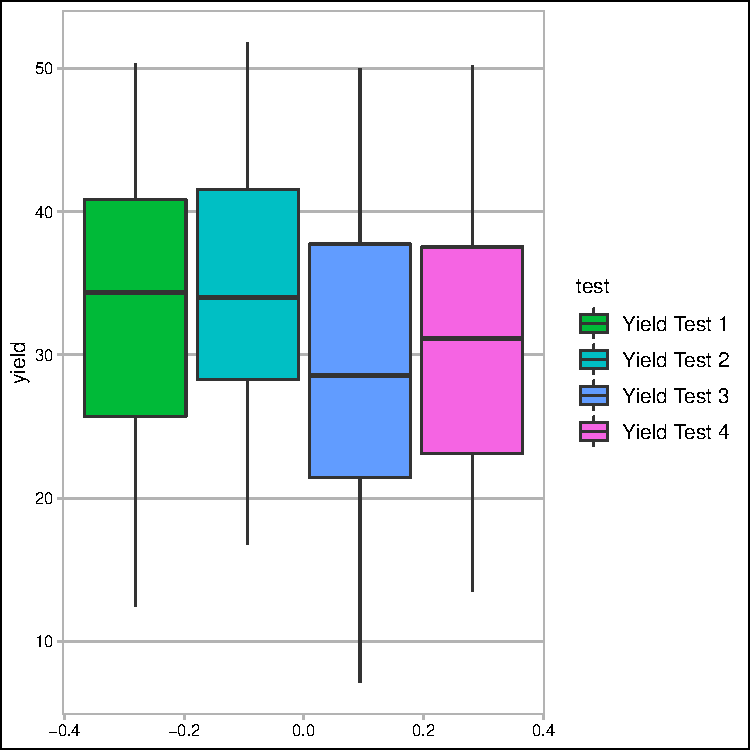
\includegraphics[width=10 cm]{C:/Users/jhgille2/Documents/R/projects/Jay_yield/exports/plots/example_plot.pdf}
\caption{This is a figure, Schemes follow the same formatting. If there are multiple panels, they should be listed as: (\textbf{a}) Description of what is contained in the first panel. (\textbf{b}) Description of what is contained in the second panel. Figures should be placed in the main text near to the first time they are cited. A caption on a single line should be centered.}
\end{figure}

\begin{figure}[H]
\centering

\includegraphics[width=3 cm]{logo-mdpi}
\caption{This is a figure, Schemes follow the same formatting. If there are multiple panels, they should be listed as: (\textbf{a}) Description of what is contained in the first panel. (\textbf{b}) Description of what is contained in the second panel. Figures should be placed in the main text near to the first time they are cited. A caption on a single line should be centered.}
\end{figure}

\begin{table}[H]
\caption{This is a table caption. Tables should be placed in the main text near to the first time they are cited.}
\centering
%% \tablesize{} %% You can specify the fontsize here, e.g.  \tablesize{\footnotesize}. If commented out \small will be used.
\begin{tabular}{ccc}
\toprule
\textbf{Title 1}    & \textbf{Title 2}  & \textbf{Title 3}\\
\midrule
entry 1     & data          & data\\
entry 2     & data          & data\\
\bottomrule
\end{tabular}
\end{table}

\begin{table}

\caption{This is a table caption. Tables should be placed in the main text near to the first time they are cited.}
\centering
\begin{tabular}[t]{lrrrrrrrrrrr}
\toprule
\textbf{ } & \textbf{mpg} & \textbf{cyl} & \textbf{disp} & \textbf{hp} & \textbf{drat} & \textbf{wt} & \textbf{qsec} & \textbf{vs} & \textbf{am} & \textbf{gear} & \textbf{carb}\\
\midrule
Mazda RX4 & 21.0 & 6 & 160 & 110 & 3.90 & 2.620 & 16.46 & 0 & 1 & 4 & 4\\
Mazda RX4 Wag & 21.0 & 6 & 160 & 110 & 3.90 & 2.875 & 17.02 & 0 & 1 & 4 & 4\\
Datsun 710 & 22.8 & 4 & 108 & 93 & 3.85 & 2.320 & 18.61 & 1 & 1 & 4 & 1\\
Hornet 4 Drive & 21.4 & 6 & 258 & 110 & 3.08 & 3.215 & 19.44 & 1 & 0 & 3 & 1\\
Hornet Sportabout & 18.7 & 8 & 360 & 175 & 3.15 & 3.440 & 17.02 & 0 & 0 & 3 & 2\\
\addlinespace
Valiant & 18.1 & 6 & 225 & 105 & 2.76 & 3.460 & 20.22 & 1 & 0 & 3 & 1\\
\bottomrule
\end{tabular}
\end{table}

This is an example of an equation:

\begin{equation}
\mathbb{S}
\end{equation}

Example of a theorem:

\begin{Theorem}
Example text of a theorem.
\end{Theorem}

The text continues here. Proofs must be formatted as follows:

Example of a proof:

\begin{proof}[Proof of Theorem 1]
Text of the proof. Note that the phrase `of Theorem 1' is optional if it is clear which theorem is being referred to.
\end{proof}

The text continues here.

\hypertarget{discussion}{%
\section{Discussion}\label{discussion}}

Authors should discuss the results and how they can be interpreted in
perspective of previous studies and of the working hypotheses. The
findings and their implications should be discussed in the broadest
context possible. Future research directions may also be highlighted.

\hypertarget{conclusion}{%
\section{Conclusion}\label{conclusion}}

This section is not mandatory, but can be added to the manuscript if the
discussion is unusually long or complex.

\hypertarget{patents}{%
\section{Patents}\label{patents}}

This section is not mandatory, but may be added if there are patents
resulting from the work reported in this manuscript.

% %%%%%%%%%%%%%%%%%%%%%%%%%%%%%%%%%%%%%%%%%%
% %% optional
% \supplementary{The following are available online at www.mdpi.com/link, Figure S1: title, Table S1: title, Video S1: title.}
%
% % Only for the journal Methods and Protocols:
% % If you wish to submit a video article, please do so with any other supplementary material.
% % \supplementary{The following are available at www.mdpi.com/link: Figure S1: title, Table S1: title, Video S1: title. A supporting video article is available at doi: link.}

\vspace{6pt}

%%%%%%%%%%%%%%%%%%%%%%%%%%%%%%%%%%%%%%%%%%
\acknowledgments{All sources of funding of the study should be
disclosed. Please clearly indicate grants that you have received in
support of your research work. Clearly state if you received funds for
covering the costs to publish in open access.}

%%%%%%%%%%%%%%%%%%%%%%%%%%%%%%%%%%%%%%%%%%
\authorcontributions{For research articles with several authors, a short
paragraph specifying their individual contributions must be provided.
The following statements should be used ``X.X. and Y.Y. conceive and
designed the experiments; X.X. performed the experiments; X.X. and Y.Y.
analyzed the data; W.W. contributed reagents/materials/analysis tools;
Y.Y. wrote the paper.'\,' Authorship must be limited to those who have
contributed substantially to the work reported.}

%%%%%%%%%%%%%%%%%%%%%%%%%%%%%%%%%%%%%%%%%%
\conflictsofinterest{Declare conflicts of interest or state `The authors
declare no conflict of interest.' Authors must identify and declare any
personal circumstances or interest that may be perceived as
inappropriately influencing the representation or interpretation of
reported research results. Any role of the funding sponsors in the
design of the study; in the collection, analyses or interpretation of
data in the writing of the manuscript, or in the decision to publish the
results must be declared in this section. If there is no role, please
state `The founding sponsors had no role in the design of the study; in
the collection, analyses, or interpretation of data; in the writing of
the manuscript, an in the decision to publish the results'.}

%%%%%%%%%%%%%%%%%%%%%%%%%%%%%%%%%%%%%%%%%%
%% optional
\abbreviations{The following abbreviations are used in this manuscript:\\

\noindent
\begin{tabular}{@{}ll}
MDPI & Multidisciplinary Digital Publishing Institute \\
DOAJ & Directory of open access journals \\
TLA & Three letter acronym \\
LD & linear dichroism \\
\end{tabular}}

\input{"appendix.tex"}

%%%%%%%%%%%%%%%%%%%%%%%%%%%%%%%%%%%%%%%%%%
% Citations and References in Supplementary files are permitted provided that they also appear in the reference list here.

%=====================================
% References, variant A: internal bibliography
%=====================================
%\reftitle{References}
%\begin{thebibliography}{999}
% Reference 1
%\bibitem[Author1(year)]{ref-journal}
%Author1, T. The title of the cited article. {\em Journal Abbreviation} {\bf 2008}, {\em 10}, 142--149.
% Reference 2
%\bibitem[Author2(year)]{ref-book}
%Author2, L. The title of the cited contribution. In {\em The Book Title}; Editor1, F., Editor2, A., Eds.; Publishing House: City, Country, 2007; pp. 32--58.
%\end{thebibliography}

% The following MDPI journals use author-date citation: Arts, Econometrics, Economies, Genealogy, Humanities, IJFS, JRFM, Laws, Religions, Risks, Social Sciences. For those journals, please follow the formatting guidelines on http://www.mdpi.com/authors/references
% To cite two works by the same author: \citeauthor{ref-journal-1a} (\citeyear{ref-journal-1a}, \citeyear{ref-journal-1b}). This produces: Whittaker (1967, 1975)
% To cite two works by the same author with specific pages: \citeauthor{ref-journal-3a} (\citeyear{ref-journal-3a}, p. 328; \citeyear{ref-journal-3b}, p.475). This produces: Wong (1999, p. 328; 2000, p. 475)

%=====================================
% References, variant B: external bibliography
%=====================================
\reftitle{References}
\externalbibliography{yes}
\bibliography{mybibfile.bib}

%%%%%%%%%%%%%%%%%%%%%%%%%%%%%%%%%%%%%%%%%%
%% optional
\sampleavailability{Samples of the compounds \ldots\ldots{} are
available from the authors.}

%% for journal Sci
%\reviewreports{\\
%Reviewer 1 comments and authors’ response\\
%Reviewer 2 comments and authors’ response\\
%Reviewer 3 comments and authors’ response
%}

%%%%%%%%%%%%%%%%%%%%%%%%%%%%%%%%%%%%%%%%%%


\end{document}
